\documentclass{article}
\usepackage{listings}
\usepackage{xcolor}
\usepackage{graphicx}

\begin{document}
\title{ACN LAB - 02 \\ Study of Wireshark Tool - Socket Programming for TCP Packets Inside UDP \\ with Simulating Packet Drop Analysis Using Wireshark}
\author{Chaitanya Talware (MIS No: 712422005) \\ Yogesh Toshniwal (MIS No: 712422021)}
\maketitle

\lstdefinestyle{python}{
    language=Python,
    basicstyle=\ttfamily\small,
    numbers=left,
    numberstyle=\tiny\color{gray},
    stepnumber=1,
    numbersep=5pt,
    backgroundcolor=\color{lightgray},
    showstringspaces=false,
    frame=single,
    rulecolor=\color{black},
    breaklines=true,
    breakatwhitespace=true,
    keywordstyle=\color{blue}\bfseries,
    commentstyle=\color{green},
    stringstyle=\color{red},
}


\section{Introduction}
This assignment demonstrates a 3-node system using Python’s socket programming. It simulates communication through TCP and UDP protocols. The system tracks packet loss and uses Wireshark to analyze network traffic. Node 1 sends data over TCP to Node 2, which forwards it over UDP to Node 3. Node 3 receives and tracks packet loss, ensuring the system models real-world network conditions effectively.
\subsection{Node 1: TCP Server}
Node 1 functions as a TCP server that listens for client connections. It receives data from a client and forwards it to Node 2 via TCP. This node generates the data packets that are sent to the next node for further processing.

\begin{itemize}
    \item Listens for UDP packets from Node 2.
    \item Tracks received packets and detects losses based on sequence numbers.
    \item Prints received and lost packet statistics.
\end{itemize}
\subsection{Node 2: TCP-to-UDP Forwarder}
Node 2 receives data from Node 1 over TCP, then forwards it to Node 3 using the UDP protocol. It simulates packet loss with a 10\% drop rate to mimic network instability, making this node an intermediary in the communication.

\begin{itemize}
    \item Receives data from Node 1 via TCP.
    \item Forwards data to Node 3 via UDP.
    \item Simulates packet loss.
\end{itemize}

\subsection{Node 3: UDP Receiver with Packet Loss Tracking}
Node 3 is responsible for receiving UDP packets from Node 2. It tracks the number of packets received and identifies lost packets by comparing the expected sequence number with the actual received packets. It prints out the total number of received and lost packets.
\begin{itemize}
    \item Listens for incoming TCP connections.
    \item Receives and forwards data to Node 2.
\end{itemize}

\subsection{Wireshark Analysis}
Wireshark is used to capture and visualize the network traffic between the nodes. It provides insights into the transmitted packets, helping confirm the packet loss and verify the system’s behavior under network conditions.
Wireshark allows us to:
\begin{itemize}
    \item Capture live network traffic in real-time.
    \item Analyze specific protocol packets such as TCP and UDP.
    \item Inspect packet contents and verify the integrity of data transmission.
    \item Track packet loss and retransmissions across the network.
\end{itemize}





\section{Source Code }
\subsection{Node 1 (Server)}
\begin{lstlisting}[style=python]

    import socket
    import time
    
    def main():
        # Set up TCP server
        server_socket = socket.socket(socket.AF_INET, socket.SOCK_STREAM)
        host = '127.0.0.1'  # Localhost
        port = 12345
        server_socket.bind((host, port))
        server_socket.listen(5)
        print(f"Node 1 (Server) listening on {host}:{port}...")
    
        while True:
            # Accept connection from Node 2
            client_socket, addr = server_socket.accept()
            print(f"Connected with Node 2 at {addr}")
    
            # Ask for sequence upper limit from user
            upper_limit = int(input("Enter upper limit for the sequence (e.g., 100): "))
    
            for i in range(1, upper_limit + 1):
                message = str(i)  # Prepare each number as a message
                client_socket.send(message.encode('utf-8'))  # Send message to Node 2
                print(f"Sent {message} to Node 2")
                time.sleep(0.5)  # Delay to simulate interval between packets
    
            print("Sequence transmission complete.")
            client_socket.send(b'q')  # Signal end of sequence
            client_socket.close()
            break  # Exit loop after one client session
    
    if __name__ == "__main__":
        main()
    

\end{lstlisting}

\subsection{Node 2 (TCP-to-UDP Forwarder)}
\begin{lstlisting}[style=python]
    # Node 2 (TCP-to-UDP Forwarder)
    import socket
    import random
    import time
    
    def main():
        # Set up TCP client to Node 1
        tcp_client = socket.socket(socket.AF_INET, socket.SOCK_STREAM)
        host = '127.0.0.1'  # IP of Node 1
        port = 12345
        tcp_client.connect((host, port))
        print("Connected to Node 1 over TCP.")
    
        # Set up UDP socket to send to Node 3
        udp_socket = socket.socket(socket.AF_INET, socket.SOCK_DGRAM)
        udp_ip = '127.0.0.1'  # IP of Node 3
        udp_port = 6000
    
        while True:
            # Receive data from Node 1 over TCP
            data = tcp_client.recv(1024).decode('utf-8')
            if data == 'q':  # Check for end of sequence
                break
            print(f"Received {data} from Node 1")
    
            # Simulate packet loss (10% drop chance)
            if random.random() < 0.1:
                print(f"Packet {data} lost (simulated).")
                continue
    
            # Forward data to Node 3 over UDP
            udp_socket.sendto(data.encode('utf-8'), (udp_ip, udp_port))
            print(f"Forwarded {data} to Node 3 via UDP")
    
            time.sleep(0.1)  # Small delay to mimic network conditions
    
        tcp_client.close()
        udp_socket.close()
    
    if __name__ == "__main__":
        main()


\end{lstlisting}



\subsection{Node 3 (UDP Receiver with Packet Loss Tracking)}
\begin{lstlisting}[style=python]

    # Node 3 (UDP Receiver with Packet Loss Tracking)
    import socket
    
    def main():
        # Set up UDP server for receiving data from Node 2
        udp_socket = socket.socket(socket.AF_INET, socket.SOCK_DGRAM)
        udp_ip = '127.0.0.1'
        udp_port = 6000
        udp_socket.bind((udp_ip, udp_port))
    
        print(f"Node 3 listening for UDP packets on {udp_ip}:{udp_port}...")
    
        received_count = 0  # Track received packets
        expected_number = 1  # Start with the first expected number
    
        while True:
            try:
                # Set a timeout for receiving packets to detect loss
                udp_socket.settimeout(5.0)
                data, addr = udp_socket.recvfrom(1024)
                number = int(data.decode('utf-8'))
                print(f"Received {number} from Node 2")
    
                # Increment received count and update expected number
                received_count += 1
    
                # Detect any missed packets between expected and received
                if number > expected_number:
                    lost_packets = number - expected_number
                    print(f"Lost {lost_packets} packets.")
                else:
                    lost_packets = 0
    
                expected_number = number + 1  # Update to the next expected number
    
            except socket.timeout:
                # If timeout occurs, assume the remaining packets are lost
                print(f"No more packets received. Assuming remaining packets lost.")
                break
    
        print(f"Total received packets: {received_count}")
        print(f"Total lost packets: {expected_number - 1 - received_count}")
    
    if __name__ == "__main__":
        main()
    

\end{lstlisting}



\section{Output}


\subsection{Images of the Program Output}
\begin{figure}[htbp]
    \centering
    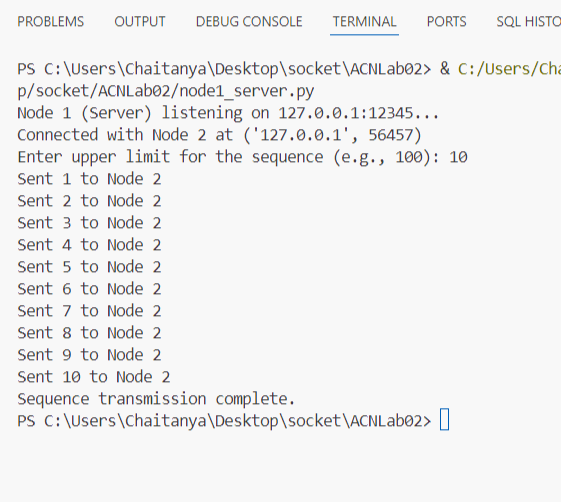
\includegraphics[]{node01.png}
    \caption{Node 1 output}
    \label{fig:node01}
\end{figure}

\begin{figure}[htbp]
    \centering
    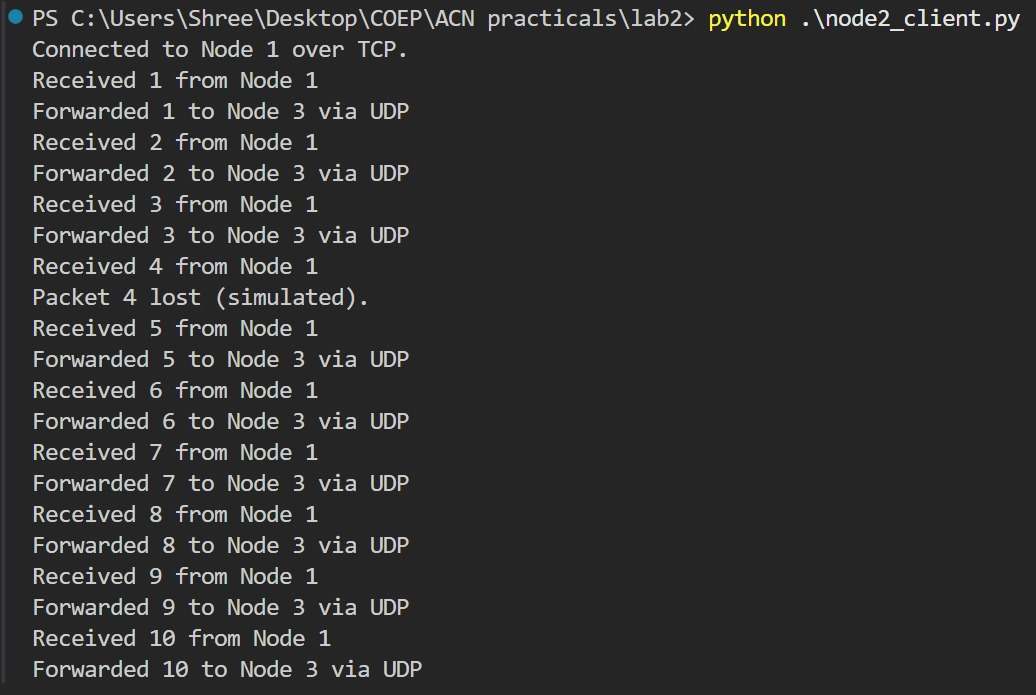
\includegraphics[angle=90,width=14cm]{node02.png}
    \caption{Node 2 output}
    \label{fig:node02}
\end{figure}

\begin{figure}[htbp]
    \centering
    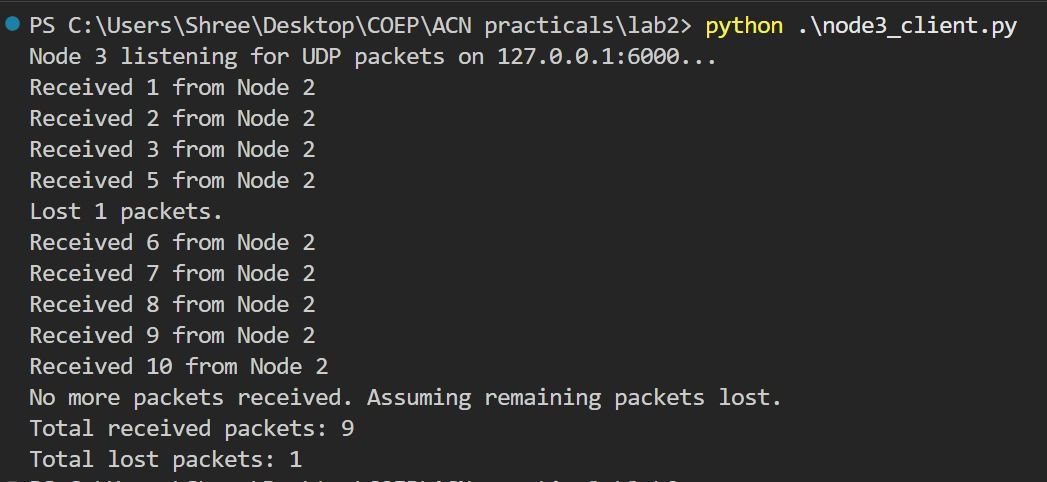
\includegraphics[angle=270,width=10cm]{node03.jpeg}
    \caption{Node 3 output}
    \label{fig:node03}
\end{figure}

\begin{figure}[htbp]
    \centering
    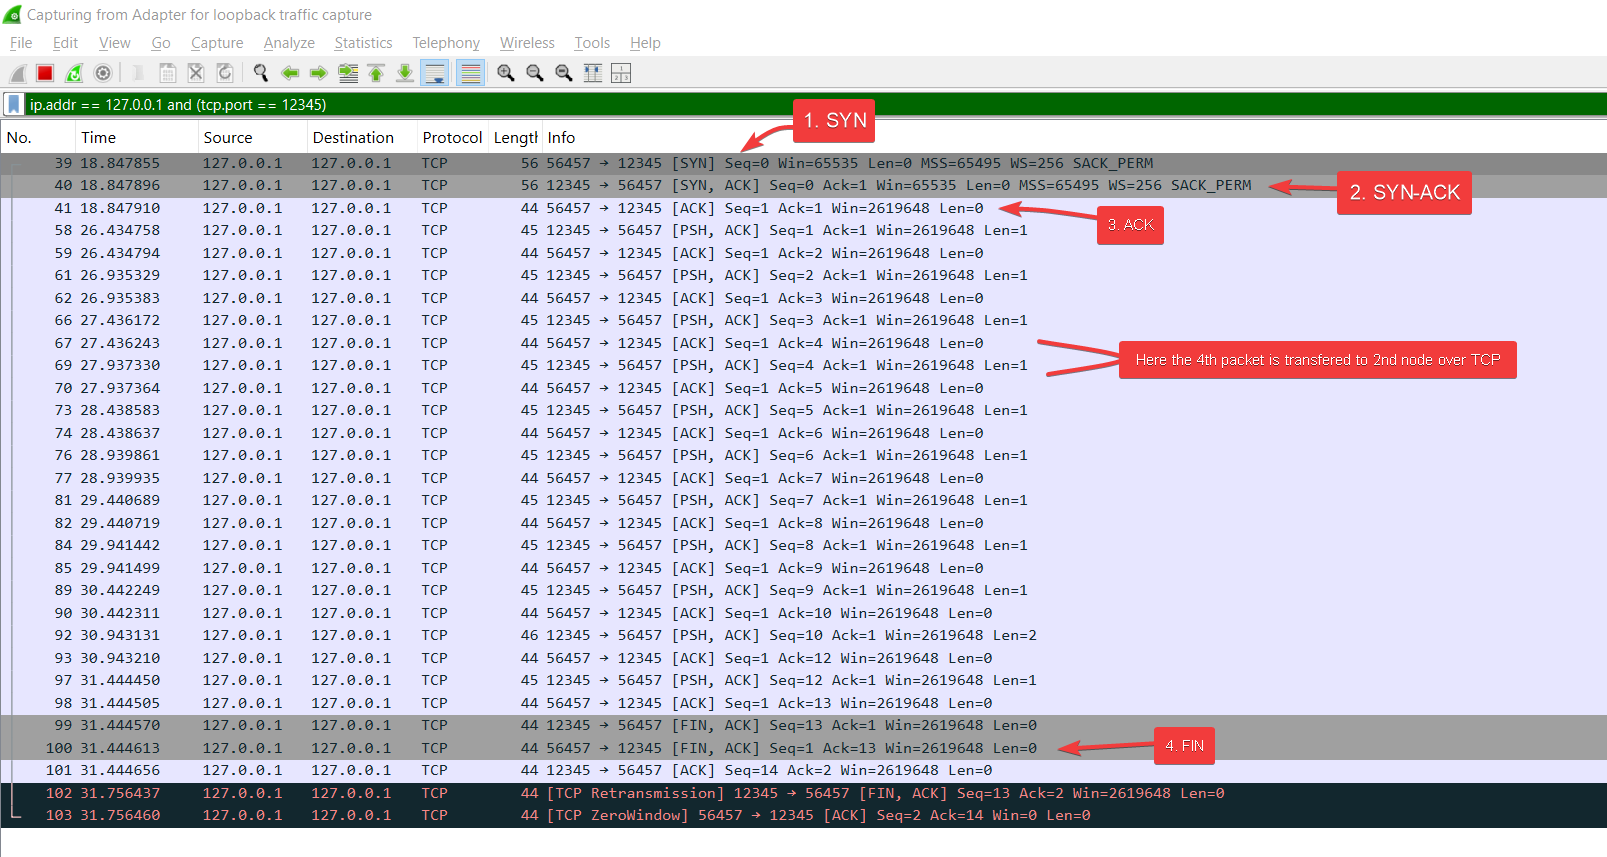
\includegraphics[angle=270,width=10cm]{WSNode1ToNode2.png}
    \caption{Wireshark Communication from Node 1 to Node 2}
    \label{fig:node1ToNode2}
\end{figure}

\begin{figure}[htbp]
    \centering
    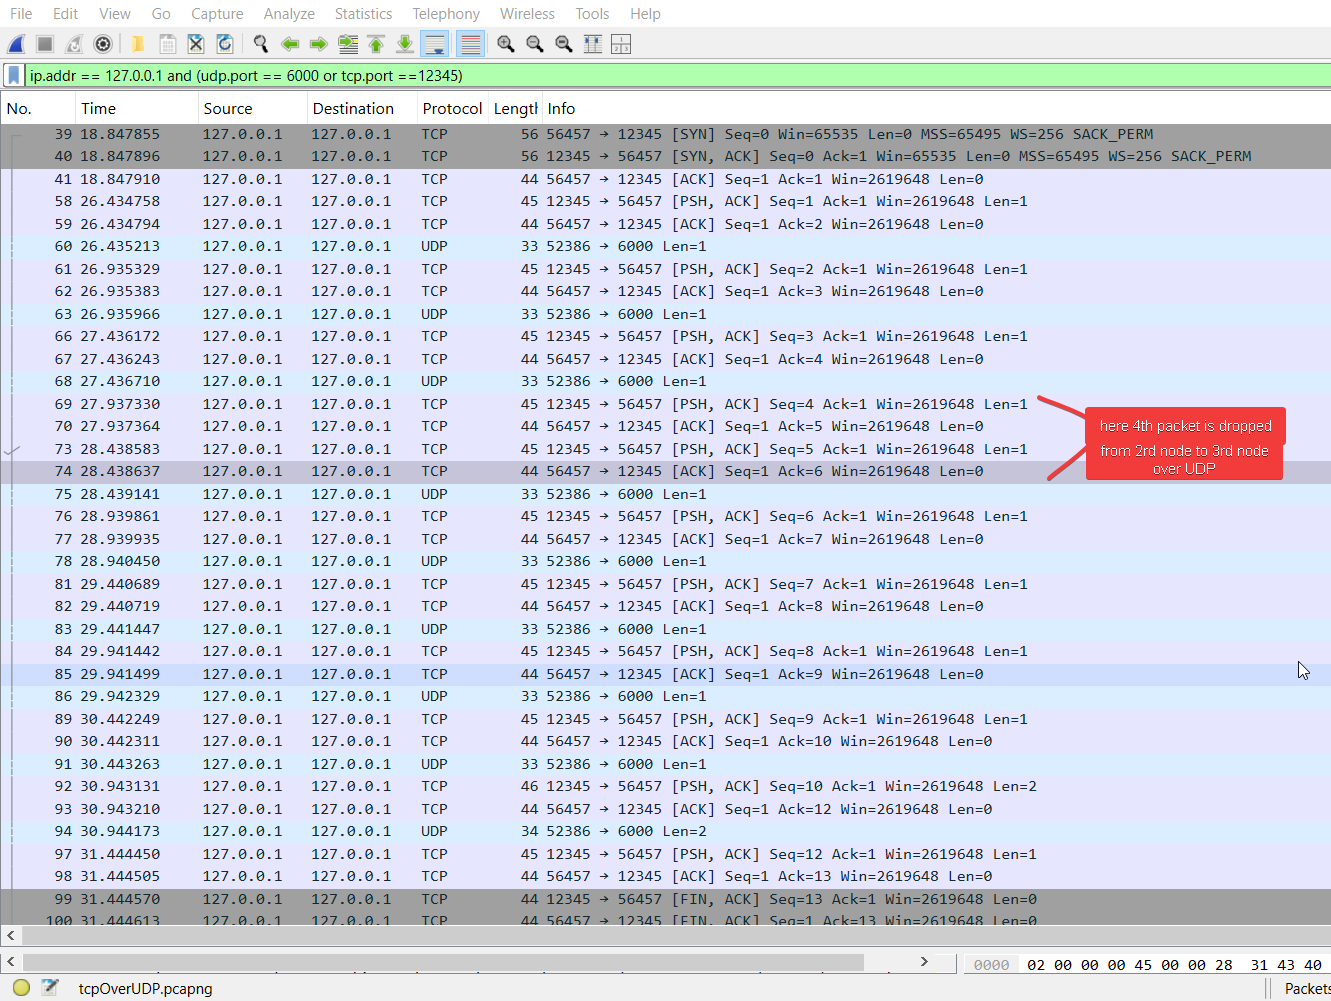
\includegraphics[angle=270,width=10cm]{WScombinedComm.png}
    \caption{Wireshark Combined Communication View}
    \label{fig:combinedComm}
\end{figure}


\begin{figure}[htbp]
    \centering
    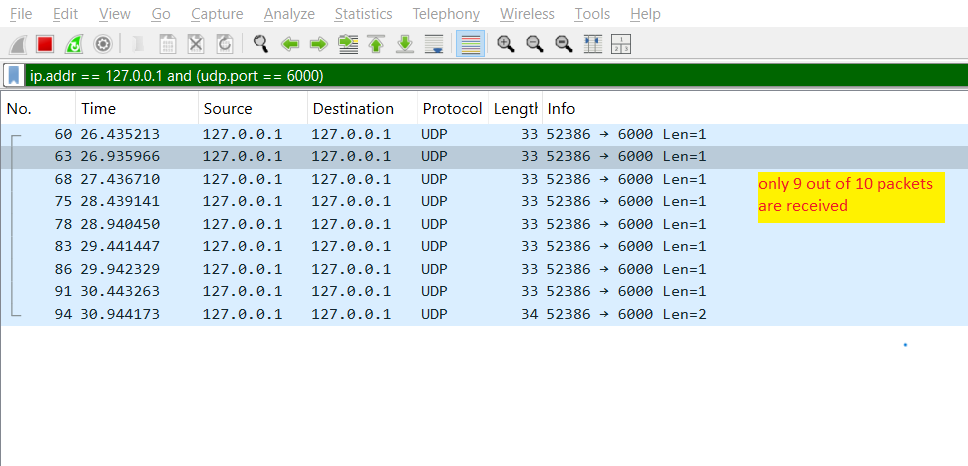
\includegraphics[angle=270,width=10cm]{WSNode2ToNode3.png}
    \caption{Wireshark Communication from Node 2 to Node 3}
    \label{fig:node2ToNode3}
\end{figure}


\end{document}
